%模板
\documentclass[a4paper]{ctexart}
\usepackage{tikz}
\usepackage{ctexcap}
\usepackage{amsmath}
\usepackage{mhchem}
\usepackage{amssymb}
\usepackage{bm}
\usepackage{unicode-math}
\usepackage[left=1.5cm,right=1.5cm,top=3cm,bottom=3cm]{geometry}
\usepackage{listings}
\usepackage{graphicx}
\usepackage{float}
\usepackage{array}
\usepackage{xcolor}

\lstset{language={[ISO]C++},tabsize=4,breaklines=true,numbers=left,backgroundcolor=\color[RGB]{245,245,244}}
\begin{document}
\begin{center}
\Huge 利用Huffman树进行文件压缩的算法和程序
\vspace{0.5cm}
\end{center}
\begin{center}
	\normalsize 郭畅 PB16070975
\end{center}
\section{代码结构}
\subsection{全局变量和常量}
\begin{lstlisting}
typedef char sourcetype;
typedef char codetype;
typedef char buffertype;

struct HuffmanNode{
sourcetype content;
int parent,lchild,rchild;
double weight;
};
const int BYTE_NUM = sizeof(sourcetype);
const int BIT_NUM = 8*BYTE_NUM;
const int CODE_TYPE_NUM = 256;//=2^BIT_NUM
const int TREE_NODE_NUM = 2*CODE_TYPE_NUM;

string InFile,OutFile;
\end{lstlisting}

\subsection{函数表}
\begin{lstlisting}[language=c++]
//Huffman Tree
void InitTree(HuffmanNode *HT,int &TreeRoot);
void DestroyTree(int &TreeRoot);
void CCreateTree(HuffmanNode *HT,int &TreeRoot);
void DCreateTree(std::string &InFile,int &TreeRoot,HuffmanNode *HT);

//compress using Huffman tree
void HCode(int *code,sourcetype source,HuffmanNode *HT,int &TreeRoot);
//decompress using Huffman tree
int HDecode(Global::buffertype buffer,Global::sourcetype &S);

int FlagFull(int flag[],int TreeRoot);
void Coding(std::string &InFile,std::string &OutFile,int &TreeRoot,HuffmanNode *HT);
void Statistic(std::string &InFile,int &TreeRoot,HuffmanNode *HT);
void Decoding(std::string &InFile,std::string &OutFile,int &TreeRoot,HuffmanNode *HT);
int main(int argc,char *argv[]);
\end{lstlisting}

\subsection{调用关系}
%\begin{minipage}{\linewidth}
\begin{figure}[H]
\centering
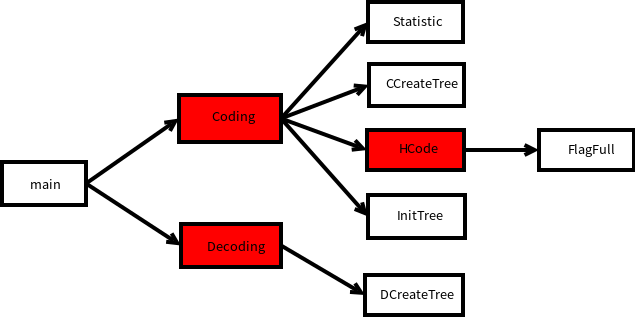
\includegraphics[width=15cm]{function_relation}
\end{figure}
%\end{minipage}

\subsection{文件结构}
\begin{figure}[H]
\begin{tabular}{|p{1.5cm}<{\centering}|p{2cm}<{\centering}|p{13cm}<{\centering}|}
	\hline
	TreeRoot & HuffmanTree & file \\
	\hline
\end{tabular}
\end{figure}
文件头前一部分为编码时使用的Huffman树相关的数据。前sizeof(TreeRoot)字节的数据存储树根的位置;之后是存储Huffman树的数组,大小为TREE\_NODE\_NUMBER*sizeof(HuffmanNode);再之后是编码的文件。压缩时先将建好的Huffman树输出到文件中,再对输入的文件进行压缩。解压时直接从文件头读取相应大小的数据块即为Huffman树,再根据Huffman树进行解压。

\section{重要代码}

\subsection{HCode}
这个函数是利用Huffman树来进行编码。得到的编码存在数组中。数组每一个元素代表一位。

\begin{lstlisting}
void HCode(int *code,sourcetype source,HuffmanNode *HT,int &TreeRoot){
	int i,j;
	int path[TREE_NODE_NUM],code_loc;
	for(code_loc=0; code_loc<CODE_TYPE_NUM; code_loc++)
	//find the location of the node
		if(HT[code_loc].content==source)
			break;
	path[0] = code_loc;//先找到被编码数所在的叶子
	i=0;
	while(HT[path[i]].parent!= -1){//依次向上寻找双亲节点直到树根
		path[i+1] = HT[path[i]].parent;
		i += 1;
	}
	//此时得到的数组path[]是逆序的编码,接下来要将编码倒过来
	if(path[i]!=TreeRoot)
		return;
	for(j=0; i>0; i--,j++){//初始时i实际上就是TreeRoot
		if(path[i-1]==HT[path[i]].lchild)//左孩子编0,右孩子编1
			code[j] = 0;
		else if(path[i-1]==HT[path[i]].rchild)
			code[j] = 1;
		}
	code[j] = -1;//最后一个元素置-1作为标志
	return;
}
\end{lstlisting}

\subsection{Coding}
这一函数当程序选择"压缩"时会被调用。

\begin{lstlisting}
void Coding(string &InFile,string &OutFile,int &TreeRoot,HuffmanNode *HT){

......

	//构造Huffman树
	InitTree(HT,TreeRoot);
	Statistic(InFile,TreeRoot,HT);
	CCreateTree(HT,TreeRoot);
	
	//begin to code the file
	int code[CODE_TYPE_NUM];
	//打开相关文件
	SourceFile.open(InFile,ios::in|ios::binary);
	CodedFile.open(OutFile,ios::out|ios::binary);
	SourceFile.clear(ios::goodbit);
	SourceFile.seekg(ios::beg);//rewind the file pointer
	void *t=&(TreeRoot);
	//将Huffman树写入压缩文件
	CodedFile.write(static_cast<char *>(t),sizeof(TreeRoot));
	t = HT;
	CodedFile.write(static_cast<char *>(t),TREE_NODE_NUM*sizeof(HuffmanNode));
	sourcetype source;//输入缓冲区
	buffertype buff;//输出缓冲区
	int buf_bit=0,i;
	while(!SourceFile.eof()){
		SourceFile.read(static_cast<char*>(&source),sizeof(source));//读取一段待压缩的编码
		HCode(code,source,HT,TreeRoot);//coding and storing in the array code;用Huffman树压缩,存储在数组code[]中
		for(i=0;code[i]!=Code_End;i++){
			if(code[i] == 1){//transform to bit如果为1
				buff <<= 1;//输出缓冲区左移一位
				buff |= 0x01;//最低位置1
				buf_bit += 1;//缓冲区占用量增加
			}//if
			else if(code[i] == 0){//如果编码为0
				buff <<= 1;//仍然左移一位
				buff &= 0xfe;//最低位置0
				buf_bit += 1;//缓冲区占用量增加
			}//else if
			//write to file
			if(buf_bit==8*sizeof(buff)){//如果缓冲区已满
				CodedFile.write(static_cast<char *>(&buff),sizeof(buff));//输出缓冲区数据
				buf_bit = 0;//缓冲区置空
			}//write to file
		}//for
	}//while
	//deal with the rest bit in buff
	while(buf_bit!=8*sizeof(buff)){//最后一个字节,缓冲区不一定满了
		buff <<= 1;//一直左移直到缓冲区满
		buf_bit ++;
	}
	CodedFile.write(static_cast<char *>(&buff),sizeof(buff));
	SourceFile.close();//输出最后一个字节的编码
	CodedFile.close();
	return;
}
\end{lstlisting}

\subsection{Decoding}
这个函数用来解压缩之前压缩的文件。

\begin{lstlisting}
void Decoding(string &InFile,string &OutFile,int &TreeRoot,HuffmanNode *HT){

......

	//构造Huffman树、打开文件
	InitTree(HT,TreeRoot);
	DCreateTree(InFile,TreeRoot,HT);
	SourceFile.open(OutFile,ios::out|ios::binary);
	CodedFile.open(InFile,ios::in|ios::binary);
	CodedFile.seekg(sizeof(TreeRoot)+TREE_NODE_NUM*sizeof(HuffmanNode),ios::beg);//指针定位到压缩文件的数据区,也就是前面文件结构的file区的开头
	
	buffertype buff;//输入缓冲区
	sourcetype decompress;//解压后编码
	int rest_bit,decom_loc;
	rest_bit = 0;
	decom_loc = TreeRoot;
	while(!CodedFile.eof()||rest_bit>0){//缓冲区还有bit位,或者文件没有结束。这两种情况都是解码未结束
		if(rest_bit==0){//输入缓冲区空,读入新数据
			CodedFile.read(static_cast<char *>(&buff),sizeof(buff));
			rest_bit = 8*sizeof(buff);
		}
		if((buff & 0x80) == 0x80)//如果最高位为1
			decom_loc = HT[decom_loc].rchild;//找右孩子
		else if((buff & 0x80) == 0x00)//如果最高位为0
			decom_loc = HT[decom_loc].lchild;//找左孩子

		if(HT[decom_loc].lchild == -1){//如果到达叶子节点
			decompress = HT[decom_loc].content;//读出解码后的数据
			SourceFile.write(static_cast<char *>(&decompress),sizeof(decompress));//写入新文件
			decom_loc = TreeRoot;//节点定位的变量回到原点(树根)
		}
			buff <<= 1;//已经解码的位左移删去
			rest_bit -= 1;//剩余位的计数减一
	}//while
	SourceFile.close();
	CodedFile.close();
	return;
}
\end{lstlisting}

\section{特殊情况}

这里所说的特殊情况,是指编/解码最后一个时的情况。

\subsection{编码(压缩)}

编码最后一个时,最后输出缓冲区可能未满。我们处理的方法是左移直到缓冲区满。比如最后一个编码出了5个位:10010,之前未输出剩余了一位0,那么还需左移2位,最后结果为:

\begin{tabular}{|c|c|c|c|c|c|c|c|}
	\hline
	0 & 1 & 0 & 0 & 1 & 0 & 0 & 0 \\ \hline
\end{tabular}

这样的编码在解码时可以进行还原。

\subsection{解码(解压)}

仍然按上面的编码,倒数第二个字节编码后,缓冲区变为

\begin{tabular}{|c|c|c|c|c|c|c|c|}
	\hline
	1 & 0 & 0 & 1 & 0 & 0 & 0 & 0\\ \hline
\end{tabular}

此时rest\_bit == 7。

再解码一个字节,状态变为:

\begin{tabular}{|c|c|c|c|c|c|c|c|}
	\hline
	0 & 0 & 0 & 0 & 0 & 0 & 0 & 0 \\ \hline
\end{tabular}

rest\_bit == 2。

再进入循环,已经到达文件尾,rest\_bit==2>0,进入循环。循环过后变为rest\_bit==1>0再进入一次,rest\_bit==0,跳出循环。最后一次的循环的数据被丢弃。而这正是我们想要的。

\section{总结}

本程序只要处理好特殊情况,基本没有什么非常困难的地方。但我的程序在编译时出现了一些问题导致无法通过编译,也没办法进行进一步的测试。这个问题等更长时间后的调试后再进行讨论。
\end{document}
